\documentclass[12pt]{beamer}
\usepackage[T1]{fontenc}
\usepackage{lmodern}
\usefonttheme{professionalfonts}
\usetheme{Madrid}
\usecolortheme{seahorse}
\usepackage[utf8]{inputenc}
\usepackage{graphicx}
\usepackage{amsmath,amssymb,mathtools}
\usepackage{listings}
\usepackage{booktabs}
\usepackage{csvsimple}
\usepackage{subcaption}
\usepackage{pgfplots}
\pgfplotsset{compat=1.18}


\title[FFT \& SVD Image Compression]{Image Compression via Cooley–Tukey FFT\\with a Brief Eckart–Young–Mirsky SVD Comparison}
\author{Tanner Wagner}
\date{6 May 2025}

% Macro for side-by-side original / compressed
\newcommand{\showCompression}[3][]{%
  \begin{columns}
    \column{0.48\textwidth}
      \includegraphics[width=\textwidth]{#2}
      \centering\footnotesize Original
    \column{0.48\textwidth}
      \includegraphics[width=\textwidth]{#3}
      \centering\footnotesize Compressed ($k=#1$)
  \end{columns}
}

\begin{document}

% Title slide
\begin{frame}
  \titlepage
\end{frame}

% Outline
\begin{frame}{Outline}
  \tableofcontents
\end{frame}

%----------------------------------------
\section{Abstract}
%----------------------------------------
\begin{frame}{Abstract}
  \begin{itemize}
    \item Design and implementation of a 2D image compressor using Cooley–Tukey FFT
    \item Frequency‐domain thresholding for significant data reduction \\
          while maintaining acceptable image quality
    \item Benchmarked on standard test images (Lena, Mandrill)
    \item Empirical runtimes follow $\mathcal{O}(M\log M)$ behavior
    \item Mathematical comparison to SVD low‐rank approximation via Eckart–Young
          highlights trade‐offs between complexity and approximation power
  \end{itemize}
\end{frame}

\section{Introduction to the Fourier Transform}

\begin{frame}{Fourier Transform (FT)}
  Define the Fourier transform operator
  \[
    \mathcal{F} : \bigl\{f\colon \mathbb{R}\to\mathbb{C}\bigr\}
    \rightarrow
    \bigl\{F\colon \mathbb{R}\to\mathbb{C}\bigr\},
  \]
  by
  \[
    (\mathcal{F}f)(\omega)
      = \int_{-\infty}^{\infty} f(t)\,e^{-i\omega t}\,dt,
    \quad \omega\in\mathbb{R}.
  \]
  Under Plancherel, $\mathcal{F}$ extends uniquely to a unitary operator on $L^2(\mathbb{R})$, with inversion
  \[
    f(t)
      = \frac{1}{2\pi}
        \int_{-\infty}^{\infty}
          (\mathcal{F}f)(\omega)\,e^{\,i\omega t}\,d\omega.
  \]
\end{frame}


%----------------------------------------
\section{Introduction to the DFT}
%----------------------------------------

\begin{frame}{Discrete Fourier Transform (DFT): Definition}
  Let \(x \in \mathbb{C}^N\).  Define the DFT operator
  \[
    F_N : \mathbb{C}^N \rightarrow \mathbb{C}^N,
    \quad
    (F_N(x))_k
      = \sum_{n=0}^{N-1} x_n \, e^{-2\pi i \tfrac{k n}{N}},
    \quad k = 0,1,\dots,N-1.
  \]
  Its inverse is
  \[
    x_n
      = \frac{1}{N}
        \sum_{k=0}^{N-1} (F_N(x))_k \, e^{2\pi i \tfrac{k n}{N}},
    \quad n = 0,1,\dots,N-1.
  \]
\end{frame}

\begin{frame}{DFT: Key Properties}
  \begin{itemize}
    \item \textbf{Linearity \& Invertibility}
    \item \textbf{Unitary up to scaling}: $F_N^*\,F_N = N\,I$
    \item \textbf{Parseval’s theorem}: 
      $\sum|x_n|^2 = \tfrac1N\sum|(F_Nx)_k|^2$
    \item \textbf{Circular convolution} in time $\leftrightarrow$ pointwise mult.\ in freq.
    \item \textbf{Conjugate symmetry} for real $x_n$: 
      $(F_Nx)_{N-k} = \overline{(F_Nx)_k}$
  \end{itemize}
\end{frame}

\section{Intuition Moving Forward}
\begin{frame}{Intuition: Why Threshold in Frequency?}
  \begin{itemize}
    \item DFT expresses $x_n$ as a sum of complex exponentials
      $\phi_k(n)=e^{-2\pi i\,kn/N}$
    \item Coeff.\ $(F_Nx)_k$ measures “energy” at frequency $k/N$
    \item Small coefficients $\Rightarrow$ little signal content
    \item Parseval’s theorem guarantees
      \[
        \sum|x_n-\tilde x_n|^2
        = \tfrac1N\sum|X_k-\tilde X_k|^2
      \]
    \item In 2D images, most energy is in low‐freq.\ modes, so zeroing high‐freq.\ easily compresses
  \end{itemize}
\end{frame}






\section{Cooley-Tukey Algorithm}
\begin{frame}{Cooley–Tukey FFT Algorithm}
  \small
  \begin{itemize}
    \item \textbf{Goal:} compute the length–\(N\) DFT in \(\mathcal{O}(N\log N)\) for \(N\) a power of two.
    \item \textbf{Divide:}
      \[
        \begin{split}
          x &= (x_0,x_1,\dots,x_{N-1})\\
            &\rightarrow
              x^{(e)}=(x_0,x_2,\dots),\quad
              x^{(o)}=(x_1,x_3,\dots).
        \end{split}
      \]
    \item \textbf{Conquer:}
      \[
        X^{(e)} = \mathrm{FFT}(x^{(e)}),\quad
        X^{(o)} = \mathrm{FFT}(x^{(o)}).
      \]
    \item \textbf{Combine:} for \(k=0,\dots,N/2-1\),
      \[
        \begin{aligned}
          X_k       &= X^{(e)}_k + \omega_N^k\,X^{(o)}_k,\\
          X_{k+N/2} &= X^{(e)}_k - \omega_N^k\,X^{(o)}_k,
        \end{aligned}
        \quad
        \omega_N=e^{-2\pi i/N}.
      \]
  \end{itemize}
\end{frame}

%---------------------------
\begin{frame}[fragile]{Cooley–Tukey FFT: Pseudocode}
  \scriptsize       % make the font tiny so it all fits
\begin{verbatim}
function FFT(x[0..N-1]):
    if N == 1:
        return x
    # split
    x_even = [ x[2*k]   for k in 0..N/2-1 ]
    x_odd  = [ x[2*k+1] for k in 0..N/2-1 ]

    # recursive calls
    E = FFT(x_even)
    O = FFT(x_odd)

    # combine
    for k from 0 to N/2-1:
        t        = exp(-2*pi*i * k / N) * O[k]
        X[k]     = E[k] + t
        X[k+N/2] = E[k] - t

    return X
\end{verbatim}
\end{frame}


% Master Theorem: statement
\begin{frame}{Master Theorem for Divide‐and‐Conquer}
  \begin{block}{Recurrence}
    \[
      T(n) \;=\; a\,T\!\bigl(\tfrac{n}{b}\bigr) \;+\; f(n),
      \quad a \ge 1,\; b > 1.
    \]
  \end{block}
  \[
    \alpha \;=\;\log_{b} a.
  \]
  \vspace{1em}
  \begin{itemize}
    \item \(f(n)\) must be asymptotically positive.
    \item We compare growth of \(f(n)\) to \(n^{\alpha}\).
  \end{itemize}
\end{frame}

\begin{frame}{Master Theorem Cases}
  \begin{block}{Let \(\alpha=\log_b a\). Then:}
    \begin{description}
      \item[\textbf{Case 1}] If \(f(n)=O(n^{\alpha-\varepsilon})\) for some \(\varepsilon>0\), then
        \[
          T(n)=\Theta(n^{\alpha}).
        \]
      \item[\textbf{Case 2}] If \(f(n)=\Theta(n^{\alpha}\log^k n)\) for some \(k\ge0\), then
        \[
          T(n)=\Theta(n^{\alpha}\log^{\,k+1}n).
        \]
      \item[\textbf{Case 3}] If 
        \(f(n)=\Omega(n^{\alpha+\varepsilon})\) for some \(\varepsilon>0\)
        and \(a\,f(n/b)\le c\,f(n)\) for some \(c<1\), then
        \[
          T(n)=\Theta(f(n)).
        \]
    \end{description}
  \end{block}
\end{frame}


%––––––––––––––––––––––––––––––––––––––––––––––––––––––––––––––––––––––––––––––––––––––––––––––
\begin{frame}{Complexity Analysis of Radix‑2 FFT}
  \begin{block}{Recurrence Relation}
    Let \(T(N)\) be the cost to compute an \(N\)-point FFT.  Then
    \[
      T(N) \;=\; 2\,T\!\bigl(\tfrac N2\bigr)\;+\;O(N).
    \]
  \end{block}

  \begin{itemize}
    \item By the Master Theorem with \(a=2\), \(b=2\), and \(f(N)=O(N)\):
      \[
        T(N) = \Theta\bigl(N\log N\bigr)
        \;\Longrightarrow\;
        \mathcal{O}(N\log N).
      \]
    \item \emph{Practical flop count:}  
      \(\tfrac N2\log_2N\) complex multiplies + \(N\log_2N\) complex adds  
      \(\;\approx\;5\,N\log_2N\) real flops.
  \end{itemize}
\end{frame}

\begin{frame}{Extension to 2D Images}
  \begin{itemize}
    \item A grayscale image of size \(M\times N\) can be viewed as an \(M\)-by-\(N\) matrix.
    \item Perform 1D FFT on each of the \(M\) rows:  
      cost \(O\bigl(N\log N\bigr)\) per row \(\;\to\;\) total \(O\bigl(M\,N\log N\bigr)\).
    \item Then perform 1D FFT on each of the \(N\) columns:  
      cost \(O\bigl(M\log M\bigr)\) per column \(\;\to\;\) total \(O\bigl(M\,N\log M\bigr)\).
    \item Overall:
      \[
        O\bigl(M\,N\log N\bigr) \;+\; O\bigl(M\,N\log M\bigr)
        \;=\;
        O\bigl(MN\log(MN)\bigr).
      \]
  \end{itemize}

  \begin{block}{Key takeaway}
    The 2D Cooley–Tukey FFT on an \(M\times N\) image runs in  
    \(\displaystyle O\bigl(MN\log(MN)\bigr)\).
  \end{block}
\end{frame}





\section{Implementation}

%––––––––––––––––––––––––––––––––––––––––––––––––––––––––––––––––––––––––––––––––––––––––––––––
\begin{frame}[fragile]{Implementation Overview}
  \begin{itemize}
    \item Written in Python using NumPy (array ops) and Pillow (I/O).
    \item Two scripts:
      \begin{itemize}
        \item \texttt{compress.py}: 2D FFT compressor (FFT → threshold → IFFT)
        \item \texttt{analyze.py}: computes MSE, PSNR, SizeRatio, SSIM and plots
      \end{itemize}
    \item All core routines from scratch.
  \end{itemize}
  \normalsize
\end{frame}

%––––––––––––––––––––––––––––––––––––––––––––––––––––––––––––––––––––––––––––––––––––––––––––––
\begin{frame}[fragile]{compress.py: Command‑line Usage}
  \begin{verbatim}
python3 compress.py input.jpg output.png --keep 0.20
  \end{verbatim}
  \normalsize
  \begin{itemize}
    \item \texttt{input.jpg}, \texttt{output.png}: file paths
    \item \texttt{--keep}: fraction of FFT coefficients to retain
  \end{itemize}
\end{frame}

%––––––––––––––––––––––––––––––––––––––––––––––––––––––––––––––––––––––––––––––––––––––––––––––
\begin{frame}[fragile]{compress.py: Load \& Resize}
  \begin{enumerate}
    \item \textbf{Load \& convert to grayscale}
\begin{lstlisting}[language=Python]
img = Image.open(input_path).convert('L')
\end{lstlisting}

    \item \textbf{Auto–resize to power‑of‑two}
\begin{lstlisting}[language=Python]
orig_w,orig_h = img.size
new_w = 2**int(floor(log2(orig_w)))
new_h = 2**int(floor(log2(orig_h)))
if (new_w,new_h) != (orig_w,orig_h):
    img = img.resize((new_w,new_h), 
    Image.LANCZOS)
\end{lstlisting}
  \end{enumerate}
  \normalsize
\end{frame}

%––––––––––––––––––––––––––––––––––––––––––––––––––––––––––––––––––––––––––––––––––––––––––––––
\begin{frame}[fragile]{compress.py: Forward FFT \& Threshold}
\begin{lstlisting}[language=Python]
def fft2d(a):
    temp = np.array([fft(row) for row in a])
    return np.array([fft(col) for col in temp.T]).T

def threshold_coeffs(A, keep_fraction):
    flat   = np.abs(A).ravel()
    n      = flat.size
    k      = max(int(np.floor(keep_fraction * n)), 1)
    thresh = np.partition(flat, -k)[-k]
    return A * (np.abs(A) >= thresh)
\end{lstlisting}
\end{frame}

%––––––––––––––––––––––––––––––––––––––––––––––––––––––––––––––––––––––––––––––––––––––––––––––
\begin{frame}[fragile]{compress.py: Inverse FFT \& Save}
\begin{lstlisting}[language=Python]
def ifft2d(A):
    temp = np.array([ifft(row) for row in A])
    return np.array([ifft(col) for col in temp.T]).T
\end{lstlisting}
\normalsize
\end{frame}



\begin{frame}{compress.py: Reconstruct}
Clip to [0,255], convert to \texttt{uint8}, and write with Pillow.\\[1ex]
The CLI parser (via Python’s \texttt{argparse}) takes
\begin{itemize}
  \item input \& output file paths
  \item \texttt{--keep} (fraction of coefficients to retain)
\end{itemize}
All in‐memory, producing standard PNG/JPEG outputs.
\end{frame}








%––––––––––––––––––––––––––––––––––––––––––––––––––––––––––––––––––––––––––––––––––––––––––––––
\begin{frame}[fragile]{Metrics \& Visualization (\texttt{analyze.py})}
\begin{lstlisting}[language=bash,breaklines=true]
python analyze.py Lena.jpeg Lena \
    --keeps 0.01 0.05 0.10 0.20 0.50 1.00
python analyze.py Mandrill.jpg Mandrill \
    --keeps 0.01 0.05 0.10 0.20 0.50 1.00
\end{lstlisting}

\begin{itemize}
  \item Load original grayscale image.
  \item For each keep–fraction, load \texttt{basename\_kXX.png} (resize if needed).
  \item Compute MSE, PSNR, SizeRatio, and (if available) SSIM.
  \item Write \texttt{metrics\_summary\_{\{basename\}}.csv} and \texttt{metrics\_summary\_{\{basename\}}.txt}.
  \item Plot \texttt{psnr\_vs\_keep.png}, \texttt{mse\_vs\_keep.png}, \texttt{size\_ratio\_vs\_keep.png}, \texttt{ssim\_vs\_keep.png}.
\end{itemize}
\end{frame}

%––––––––––––––––––––––––––––––––––––––––––––––––––––––––––––––––––––––––––––––––––––––––––––––
\begin{frame}[fragile]{analyze.py Pseudocode}
\scriptsize
\begin{verbatim}
function analyze_metrics(orig, basename, keeps):
    I = load_grayscale(orig)
    results = []
    for k in keeps:
        I_k   = load_image(f"{basename}_k{k}.png")
        mse   = mean((I - I_k)**2)
        psnr  = 10 * log10(MAX**2 / mse)
        ssim  = compute_ssim(I, I_k)
        size  = filesize(I_k) / filesize(orig)
        results.append((k, mse, psnr, size, ssim))

    write_csv(
      f"metrics_summary_{basename}.csv", 
      results
    )
    plot_vs_keep(results)
\end{verbatim}
\normalsize
\end{frame}

%––––––––––––––––––––––––––––––––––––––––––––––––––––––––––––––––––––––––––––––––––––––––––––––
\begin{frame}[fragile]{Project Directory Structure}
\scriptsize
\begin{verbatim}
FINAL_PROJECT/
|-- compress.py
|-- analyze.py
|-- benchmark_images.py       # timing script
|-- Lena.jpeg
|-- Mandrill.jpg             # original test images
|-- Lena_k0.01.png … Lena_k1.00.png
|-- Mandrill_k0.01.png … Mandrill_k1.00.png
|-- metrics_summary_Lena.csv/.txt
|-- metrics_summary_Mandrill.csv/.txt
|-- psnr_vs_keep_*.png
|-- mse_vs_keep_*.png
|-- size_ratio_vs_keep_*.png
|-- ssim_vs_keep_*.png
|-- benchmark_images_Lena.csv/.txt
|-- benchmark_images_Mandrill.csv/.txt
|-- time_vs_M_*.png
`-- time_vs_MlogM_*.png
\end{verbatim}
\normalsize
\end{frame}












\section{Experimental Setup}

\begin{frame}{Test Images}
I evaluated my compressor on two standard $256 \times 256$ grayscale images:
  \begin{itemize}
    \item \textbf{Lena} (\texttt{Lena.jpeg}): a portrait with smooth regions and fine detail in hair and hat.
    \item \textbf{Mandrill} (\texttt{Mandrill.jpg}): a baboon face image with high‑frequency texture in fur and foliage.
  \end{itemize}

  Both images were converted to single‑channel (grayscale) and confirmed to be \(256\times256\) pixels.
\end{frame}


\begin{frame}[fragile]{Compression Procedure}
  \begin{itemize}
    \item Generated compressed outputs at six keep‑fractions
      \(\{0.01,0.05,0.10,0.20,0.50,1.00\}\).
    \item For each \(k\), run in your project directory:
  \end{itemize}

  \begin{block}{Shell Loop}
\begin{verbatim}
for k in 0.01 0.05 0.10 0.20 0.50 1.00; do
  python3 compress.py Lena.jpeg    Lena_k${k}.png    
  --keep $k
  python3 compress.py Mandrill.jpg Mandrill_k${k}.png 
  --keep $k
done
\end{verbatim}
  \end{block}

  This produces, e.g., \texttt{Lena\_k0.01.png}, …, \texttt{Lena\_k1.00.png} (and likewise for Mandrill).
\end{frame}




\begin{frame}[fragile]{Analysis Procedure}
  \begin{block}{Run analysis}
\begin{verbatim}
python3 analyze.py Lena.jpeg    Lena
python3 analyze.py Mandrill.jpg Mandrill
\end{verbatim}
  \end{block}

  Each invocation reads the original plus its six compressed variants and produces:
  \begin{itemize}
    \item \texttt{metrics\_summary.csv} \quad (comma‐delimited table of keep, MSE, PSNR, SizeRatio, [SSIM])  
    \item \texttt{metrics\_summary.txt} \quad (tab‐delimited version)  
    \item \texttt{psnr\_vs\_keep.png}  
    \item \texttt{mse\_vs\_keep.png}  
    \item \texttt{size\_ratio\_vs\_keep.png}  
    \item \texttt{ssim\_vs\_keep.png} \quad (if \texttt{scikit‑image} is installed)  
  \end{itemize}
\end{frame}






\begin{frame}[fragile]{Benchmarking Procedure}
  \small
  To confirm the \(\Theta(M\log M)\) scaling, I resized each image to \(n \times n\) for 
  \(n \in \{64,128,256,512\}\) and ran:
  \begin{block}{Timing commands}
\begin{verbatim}
python3 benchmark_images.py Lena.jpeg    --keep 0.20 
--sizes 64 128 256 512
python3 benchmark_images.py Mandrill.jpg --keep 0.20 
--sizes 64 128 256 512
\end{verbatim}
  \end{block}
  This produced:
  \begin{itemize}
    \item \texttt{benchmark\_images.csv}   — table of \(n\), \(M=n^2\), time, and \(M\log_2M\)  
    \item \texttt{time\_vs\_M.png}  
    \item \texttt{time\_vs\_MlogM.png}  
  \end{itemize}
\end{frame}












% --------------------------------------------------------
% Quality Metrics Overview
% --------------------------------------------------------
\begin{frame}{Quality Metrics}
  \begin{itemize}
    \item Mean Squared Error (MSE)
    \item Peak Signal‑to‑Noise Ratio (PSNR)
    \item Structural Similarity Index (SSIM)
    \item Compression Ratio (SizeRatio)
  \end{itemize}
\end{frame}

% --------------------------------------------------------
% Mean Squared Error
% --------------------------------------------------------
\begin{frame}{Mean Squared Error (MSE)}
  \[
    \mathrm{MSE}(I,\tilde I)
    = \frac{1}{MN} \sum_{i=1}^M \sum_{j=1}^N \bigl(I_{i,j} - \tilde I_{i,j}\bigr)^2
  \]
  \vspace{1em}
  \begin{itemize}
    \item Monotonic decrease as keep‑fraction \(k\) increases.
    \item Example values:
      \begin{itemize}
        \item \(k=0.01\): \(\mathrm{MSE}\sim10^3\)
        \item \(k=1.00\): \(\mathrm{MSE}\approx0\)
      \end{itemize}
  \end{itemize}
\end{frame}

% --------------------------------------------------------
% Peak Signal-to-Noise Ratio
% --------------------------------------------------------
\begin{frame}{Peak Signal‑to‑Noise Ratio (PSNR)}
  \[
    \mathrm{PSNR}(I,\tilde I)
    = 10 \,\log_{10}\!\Bigl(\frac{\mathrm{MAX}^2}{\mathrm{MSE}}\Bigr),
    \quad \mathrm{MAX}=255
  \]
  \vspace{1em}
  \begin{itemize}
    \item Higher PSNR ⇒ better fidelity.
    \item Visually lossless threshold: \(\mathrm{PSNR}\ge30\)\,dB.
    \item Expectation:
      \begin{itemize}
        \item \(k\ge0.20\) ⇒ \(\mathrm{PSNR}\gtrsim30\)\,dB
        \item \(k=1.00\) ⇒ \(\mathrm{PSNR}\sim50\)\,dB
      \end{itemize}
  \end{itemize}
\end{frame}

% --------------------------------------------------------
% Structural Similarity Index
% --------------------------------------------------------
\begin{frame}{Structural Similarity Index (SSIM)}
  \[
    \mathrm{SSIM}(I,\tilde I)
    = \frac{(2\mu_I\mu_{\tilde I}+C_1)\,(2\sigma_{I\tilde I}+C_2)}
           {(\mu_I^2 + \mu_{\tilde I}^2 + C_1)\,(\sigma_I^2 + \sigma_{\tilde I}^2 + C_2)}
  \]
  \vspace{1em}
  \begin{itemize}
    \item Perceptual similarity metric in \([0,1]\).
    \item Low (\(\sim0.2\!-\!0.4\)) at \(k=0.01\), approaches \(1.0\) as \(k\to1\).
    \item Complements PSNR by modeling human perception.
  \end{itemize}
\end{frame}

% --------------------------------------------------------
% Compression Ratio
% --------------------------------------------------------
\begin{frame}{Compression Ratio (SizeRatio)}
  \[
    \mathrm{SizeRatio}(k)
    = \frac{\text{size of compressed file at }k}
           {\text{size of original file}}
  \]
  \vspace{1em}
  \begin{itemize}
    \item Ideal: linear in \(k\).
    \item Empirical (PNG vs.\ JPEG original):
      \begin{itemize}
        \item Rapid growth for small \(k\).
        \item Flattens out for larger \(k\) (format overhead, entropy).
      \end{itemize}
  \end{itemize}
\end{frame}



% --------------------------------------------------------
% Expected Plots
% --------------------------------------------------------
\begin{frame}{Expected Plots}
  \begin{itemize}
    \item \textbf{MSE vs.\ \(k\)}  
      \begin{itemize}
        \item Steeply decreasing, convex curve
      \end{itemize}
    \item \textbf{PSNR vs.\ \(k\)}  
      \begin{itemize}
        \item Increasing, with diminishing returns (concave)
      \end{itemize}
    \item \textbf{SizeRatio vs.\ \(k\)}  
      \begin{itemize}
        \item \emph{Theoretical:} straight line \(y = k\)  
        \item \emph{Empirical:} rapid growth for \(0 \le k \le 0.2\), then slower, flattening increase  
      \end{itemize}
  \end{itemize}

  \vspace{1em}
  \noindent These curves illustrate the trade‑off:
  \(\uparrow\) quality (PSNR, SSIM) vs.\ \(\downarrow\) compression (SizeRatio), with MSE as an error metric.
\end{frame}






\section{Results}

\begin{frame}{Visual Compression Results}
For each test image (Lena and Mandrill) we'll look at the original (left) and the compressor output (right) at keep-fractions $k \in \{0.01,0.05,0.10,0.20,0.50,1.00\}$
\end{frame}

%---- Lena slides ----
\begin{frame}{Lena, \(k=0.01\)}
  \begin{columns}
    \column{0.48\textwidth}
      \centering
      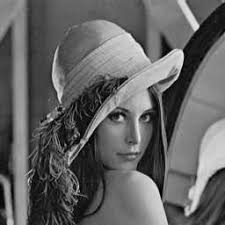
\includegraphics[width=\textwidth]{Lena.jpeg}\\
      \footnotesize Original
    \column{0.48\textwidth}
      \centering
      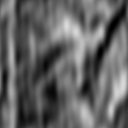
\includegraphics[width=\textwidth]{Lena_k01.png}\\
      \footnotesize Compressed, \(k=0.01\)
  \end{columns}
\end{frame}

\begin{frame}{Lena, \(k=0.05\)}
  \begin{columns}
    \column{0.48\textwidth}
      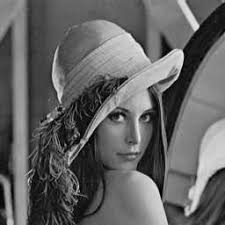
\includegraphics[width=\textwidth]{Lena.jpeg}\\
      \footnotesize Original
    \column{0.48\textwidth}
      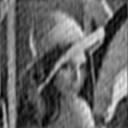
\includegraphics[width=\textwidth]{Lena_k05.png}\\
      \footnotesize Compressed, \(k=0.05\)
  \end{columns}
\end{frame}

\begin{frame}{Lena, \(k=0.10\)}
  \begin{columns}
    \column{0.48\textwidth}
      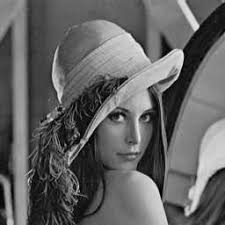
\includegraphics[width=\textwidth]{Lena.jpeg}\\
      \footnotesize Original
    \column{0.48\textwidth}
      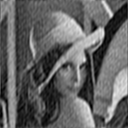
\includegraphics[width=\textwidth]{Lena_k10.png}\\
      \footnotesize Compressed, \(k=0.10\)
  \end{columns}
\end{frame}

\begin{frame}{Lena, \(k=0.20\)}
  \begin{columns}
    \column{0.48\textwidth}
      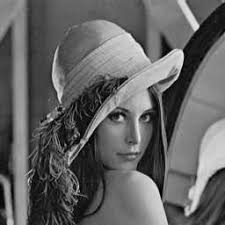
\includegraphics[width=\textwidth]{Lena.jpeg}\\
      \footnotesize Original
    \column{0.48\textwidth}
      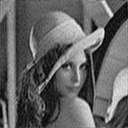
\includegraphics[width=\textwidth]{Lena_k20.png}\\
      \footnotesize Compressed, \(k=0.20\)
  \end{columns}
\end{frame}

\begin{frame}{Lena, \(k=0.50\)}
  \begin{columns}
    \column{0.48\textwidth}
      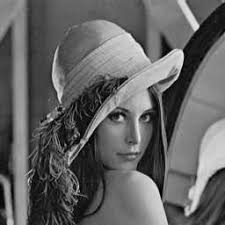
\includegraphics[width=\textwidth]{Lena.jpeg}\\
      \footnotesize Original
    \column{0.48\textwidth}
      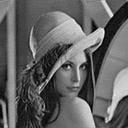
\includegraphics[width=\textwidth]{Lena_k50.png}\\
      \footnotesize Compressed, \(k=0.50\)
  \end{columns}
\end{frame}

\begin{frame}{Lena, \(k=1.00\)}
  \begin{columns}
    \column{0.48\textwidth}
      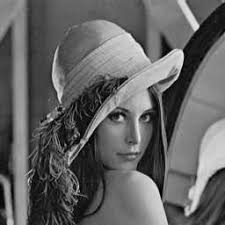
\includegraphics[width=\textwidth]{Lena.jpeg}\\
      \footnotesize Original
    \column{0.48\textwidth}
      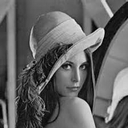
\includegraphics[width=\textwidth]{Lena_k100.png}\\
      \footnotesize Compressed, \(k=1.00\)
  \end{columns}
\end{frame}

%---- Mandrill slides ----
\begin{frame}{Mandrill, \(k=0.01\)}
  \begin{columns}
    \column{0.48\textwidth}
      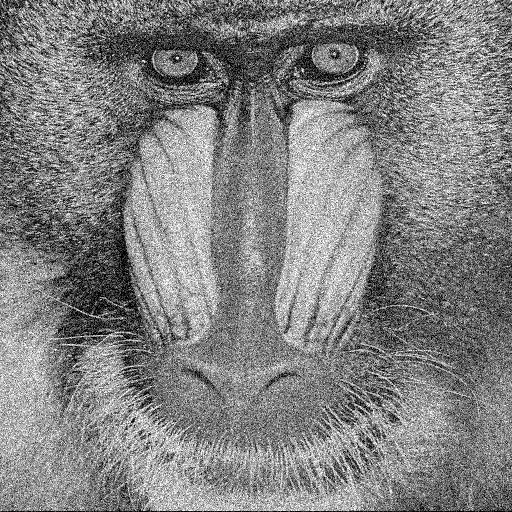
\includegraphics[width=\textwidth]{Mandrill.jpg}\\
      \footnotesize Original
    \column{0.48\textwidth}
      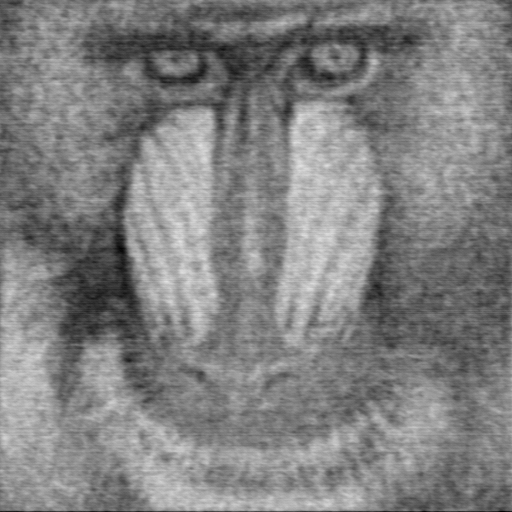
\includegraphics[width=\textwidth]{Mandrill_k01.png}\\
      \footnotesize Compressed, \(k=0.01\)
  \end{columns}
\end{frame}

\begin{frame}{Mandrill, \(k=0.05\)}
  \begin{columns}
    \column{0.48\textwidth}
      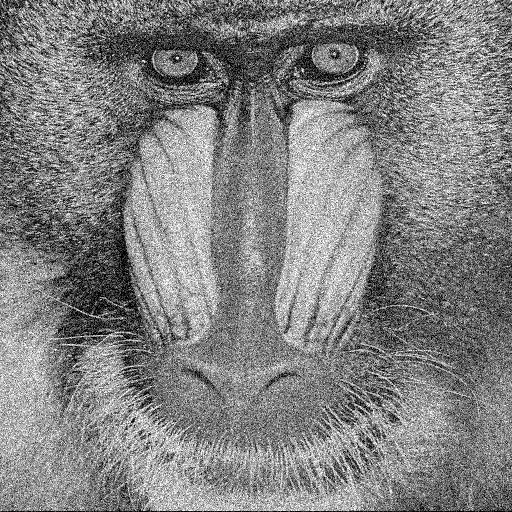
\includegraphics[width=\textwidth]{Mandrill.jpg}\\
      \footnotesize Original
    \column{0.48\textwidth}
      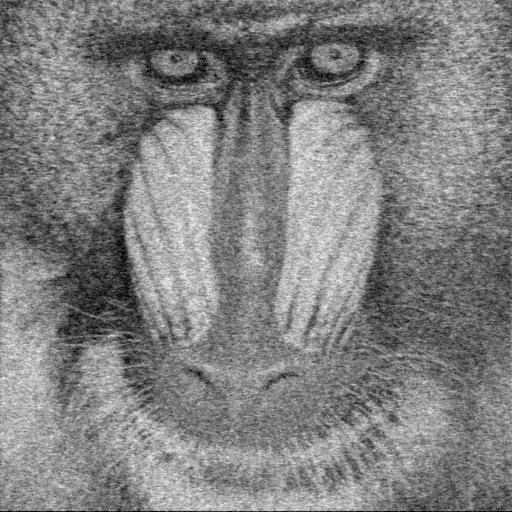
\includegraphics[width=\textwidth]{Mandrill_k05.png}\\
      \footnotesize Compressed, \(k=0.05\)
  \end{columns}
\end{frame}

\begin{frame}{Mandrill, \(k=0.10\)}
  \begin{columns}
    \column{0.48\textwidth}
      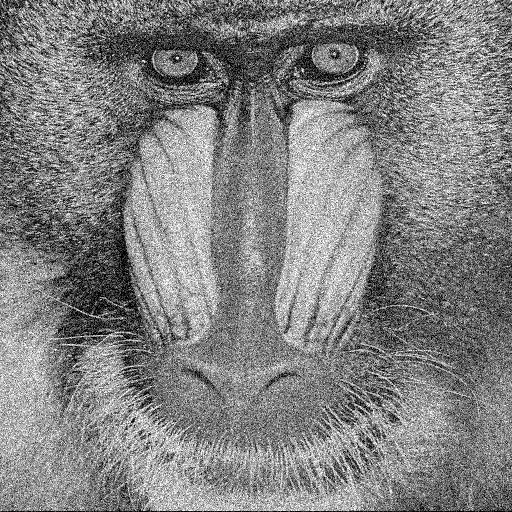
\includegraphics[width=\textwidth]{Mandrill.jpg}\\
      \footnotesize Original
    \column{0.48\textwidth}
      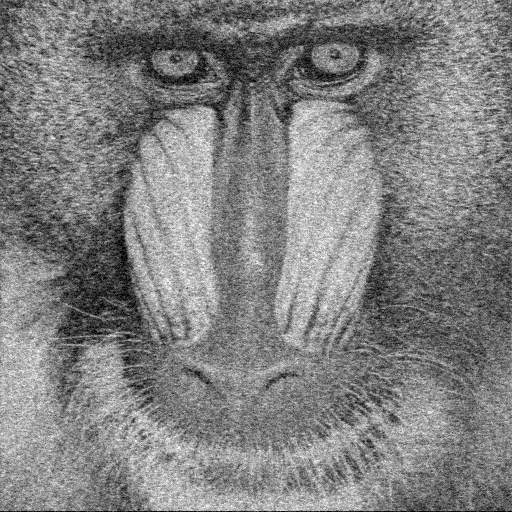
\includegraphics[width=\textwidth]{Mandrill_k10.png}\\
      \footnotesize Compressed, \(k=0.10\)
  \end{columns}
\end{frame}

\begin{frame}{Mandrill, \(k=0.20\)}
  \begin{columns}
    \column{0.48\textwidth}
      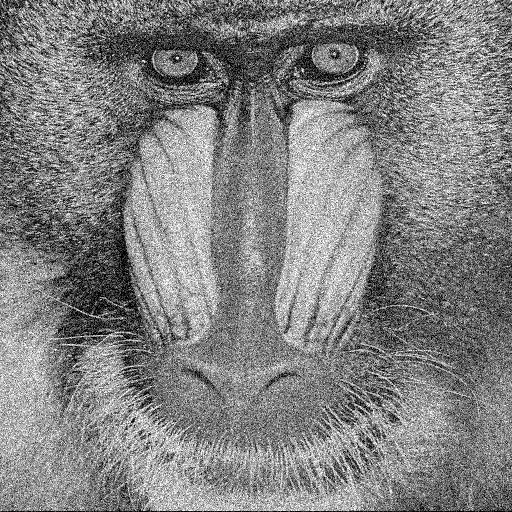
\includegraphics[width=\textwidth]{Mandrill.jpg}\\
      \footnotesize Original
    \column{0.48\textwidth}
      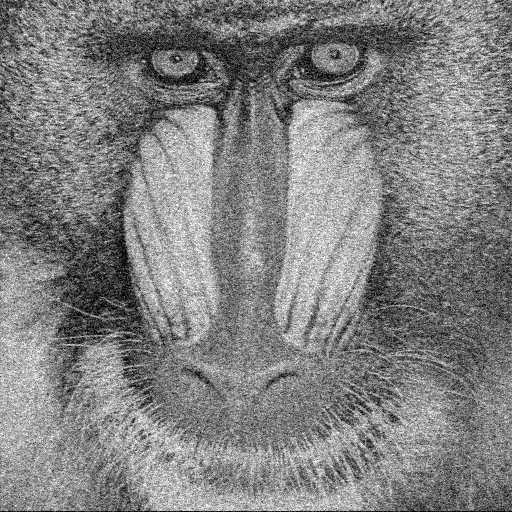
\includegraphics[width=\textwidth]{Mandrill_k20.png}\\
      \footnotesize Compressed, \(k=0.20\)
  \end{columns}
\end{frame}

\begin{frame}{Mandrill, \(k=0.50\)}
  \begin{columns}
    \column{0.48\textwidth}
      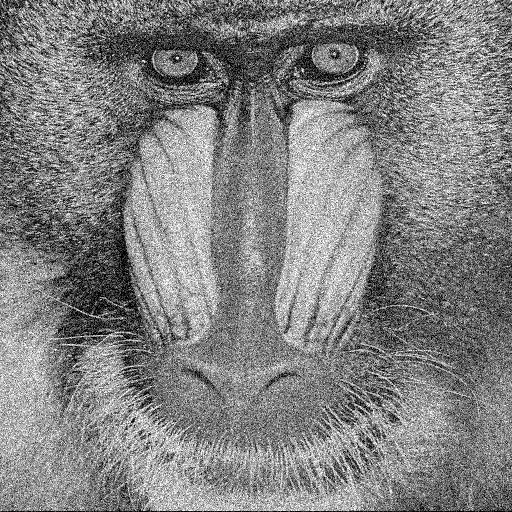
\includegraphics[width=\textwidth]{Mandrill.jpg}\\
      \footnotesize Original
    \column{0.48\textwidth}
      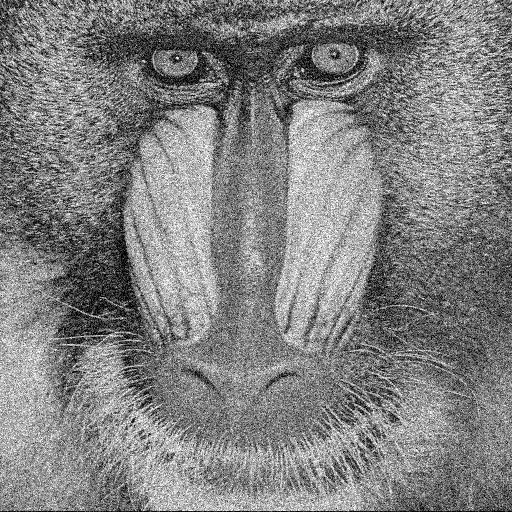
\includegraphics[width=\textwidth]{Mandrill_k50.png}\\
      \footnotesize Compressed, \(k=0.50\)
  \end{columns}
\end{frame}

\begin{frame}{Mandrill, \(k=1.00\)}
  \begin{columns}
    \column{0.48\textwidth}
      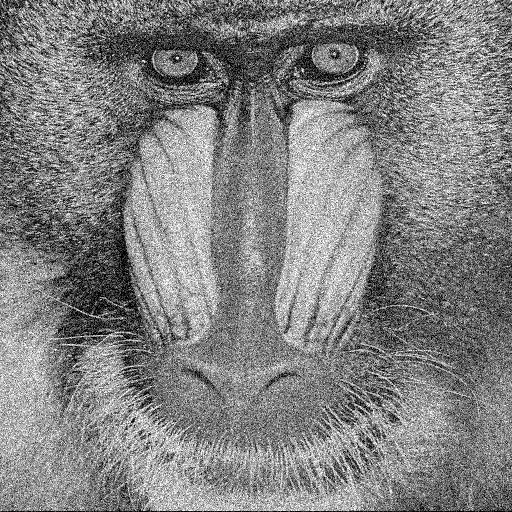
\includegraphics[width=\textwidth]{Mandrill.jpg}\\
      \footnotesize Original
    \column{0.48\textwidth}
      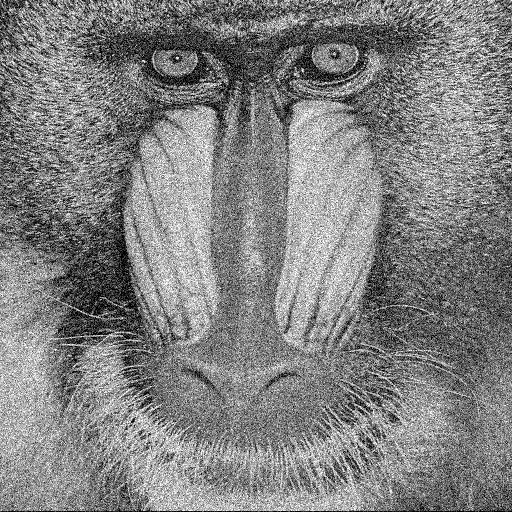
\includegraphics[width=\textwidth]{Mandrill_k100.png}\\
      \footnotesize Compressed, \(k=1.00\)
  \end{columns}
\end{frame}

%–––––––––––––––––––––––––––
\begin{frame}[fragile]{Lena: Quality Metrics Table}
  \scriptsize
  \centering
  \csvautobooktabular{metrics_summary_Lena.csv}
\end{frame}

%–––––––––––––––––––––––––––
\begin{frame}{Lena: PSNR vs.\ keep–fraction}
  \centering
  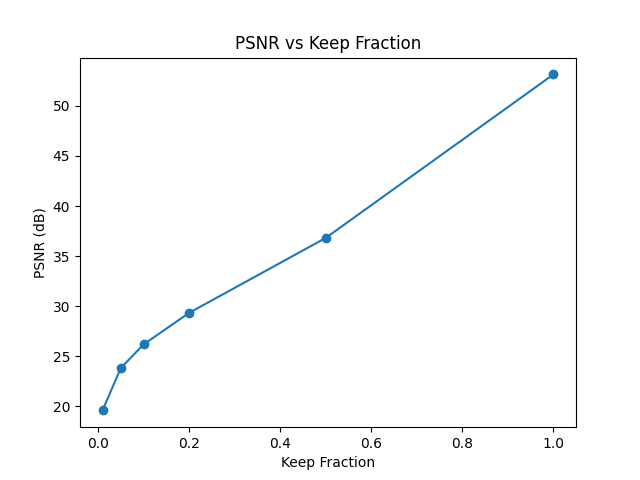
\includegraphics[width=0.8\textwidth]{psnr_vs_keep_Lena.png}
\end{frame}

%–––––––––––––––––––––––––––
\begin{frame}{Lena: MSE vs.\ keep–fraction}
  \centering
  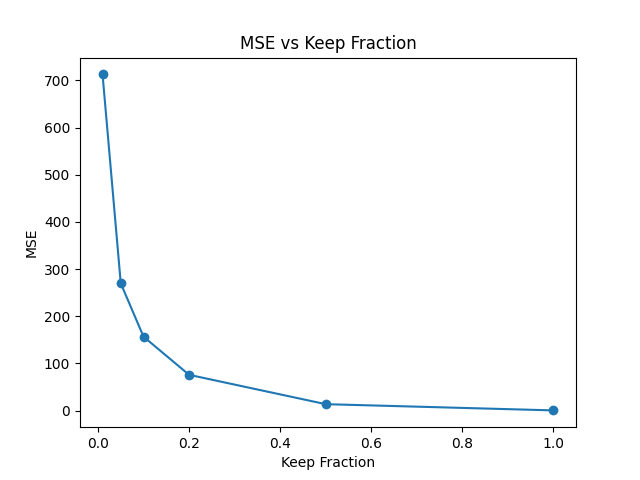
\includegraphics[width=0.8\textwidth]{mse_vs_keep_Lena.png}
\end{frame}

%–––––––––––––––––––––––––––
\begin{frame}{Lena: Empirical SizeRatio vs.\ keep–fraction}
  \centering
  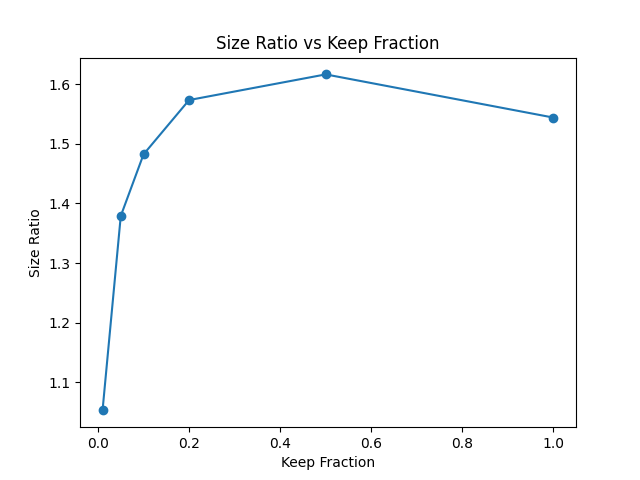
\includegraphics[width=0.8\textwidth]{size_ratio_vs_keep_Lena.png}
\end{frame}

%–––––––––––––––––––––––––––
\begin{frame}{Lena: SSIM vs.\ keep–fraction}
  \centering
  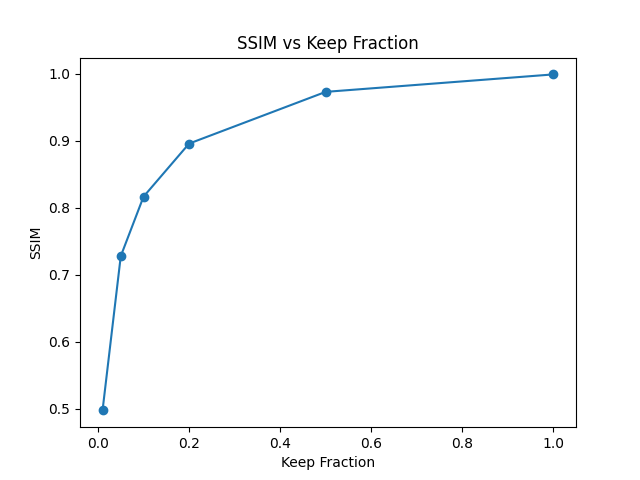
\includegraphics[width=0.8\textwidth]{ssim_vs_keep_Lena.png}
\end{frame}


%–––––––––––––––––––––––––––
\begin{frame}[fragile]{Mandrill: Quality Metrics Table}
  \scriptsize
  \centering
  \csvautobooktabular{metrics_summary_Mandrill.csv}
\end{frame}

%–––––––––––––––––––––––––––
\begin{frame}{Mandrill: PSNR vs.\ keep–fraction}
  \centering
  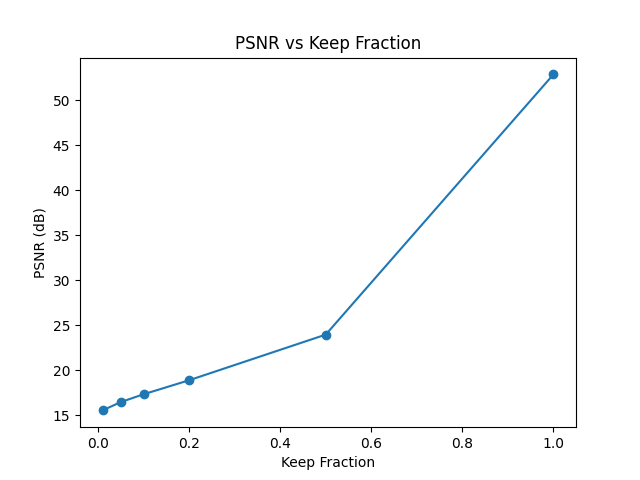
\includegraphics[width=0.8\textwidth]{psnr_vs_keep_Mandrill.png}
\end{frame}

%–––––––––––––––––––––––––––
\begin{frame}{Mandrill: MSE vs.\ keep–fraction}
  \centering
  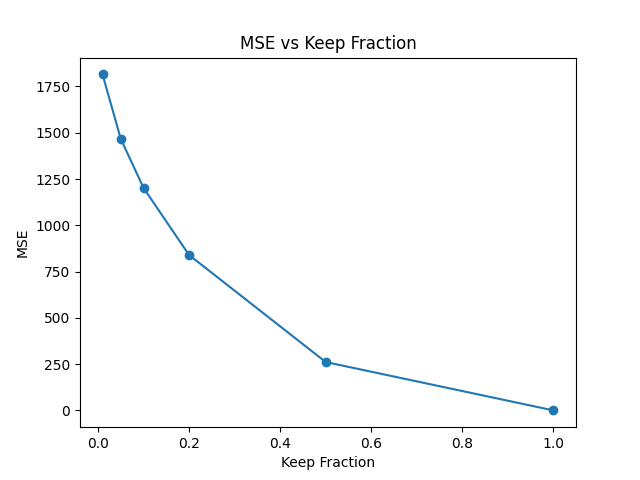
\includegraphics[width=0.8\textwidth]{mse_vs_keep_Mandrill.png}
\end{frame}

%–––––––––––––––––––––––––––
\begin{frame}{Mandrill: Empirical SizeRatio vs.\ keep–fraction}
  \centering
  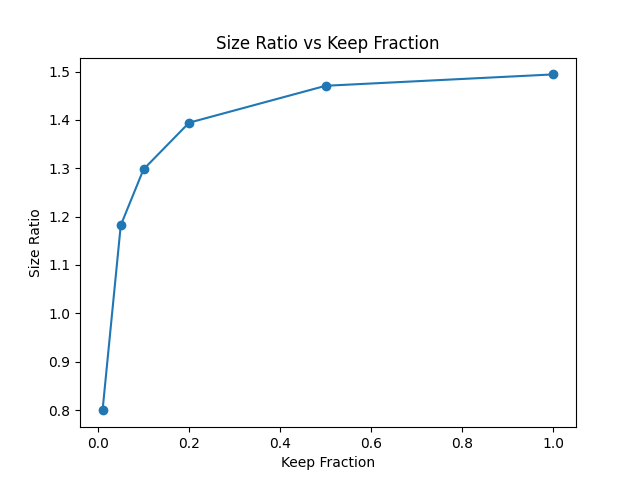
\includegraphics[width=0.8\textwidth]{size_ratio_vs_keep_Mandrill.png}
\end{frame}

%–––––––––––––––––––––––––––
\begin{frame}{Mandrill: SSIM vs.\ keep–fraction}
  \centering
  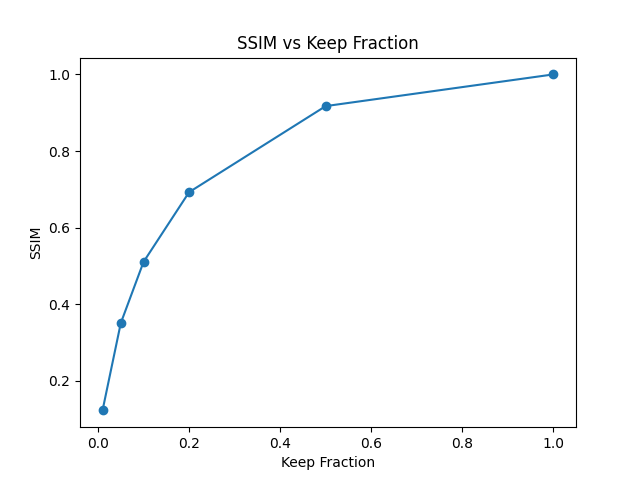
\includegraphics[width=0.8\textwidth]{ssim_vs_keep_Mandrill.png}
\end{frame}


%––––––––––––––––––––––––––––––––––––––––––––––––––––––––––––––––––––––––––––––––––––––––––––––
\begin{frame}{Summary of Results: Lena}
  \begin{itemize}
    \item \textbf{PSNR vs.\ \(k\)}: nearly linear, from \(19.6\)\,dB at \(k=0.01\) to \(53.1\)\,dB at \(k=1.00\), slight curvature at low \(k\).
    \item \textbf{MSE vs.\ \(k\)}: rapid drop from \(712.9\) to \(0.32\), flattens for \(k\ge0.5\).
    \item \textbf{SizeRatio vs.\ \(k\)}: grows quickly for \(k\le0.2\) then tapers off (log‐like) despite underlying linear coefficient count.
    \item \textbf{SSIM vs.\ \(k\)}: sigmoidal rise from \(0.50\) at \(k=0.01\) to \(0.999\) at \(k=1.00\), tracking PSNR.
  \end{itemize}
\end{frame}

%––––––––––––––––––––––––––––––––––––––––––––––––––––––––––––––––––––––––––––––––––––––––––––––
\begin{frame}{Summary of Results: Mandrill}
  \begin{itemize}
    \item \textbf{PSNR vs.\ \(k\)}: from \(15.54\)\,dB at \(k=0.01\) to \(52.85\)\,dB at \(k=1.00\), with a pronounced “kink” near \(k=0.5\).
    \item \textbf{MSE vs.\ \(k\)}: drops from \(1815.0\) to \(0.34\), flattening for higher \(k\).
    \item \textbf{SizeRatio vs.\ \(k\)}: same rapid‐then‐flatten behavior as Lena.
    \item \textbf{SSIM vs.\ \(k\)}: climbs from \(0.12\) to nearly \(1.00\), indicating sharp fidelity improvement once enough spectrum is retained.
  \end{itemize}
\end{frame}

%––––––––––––––––––––––––––––––––––––––––––––––––––––––––––––––––––––––––––––––––––––––––––––––
\begin{frame}{Overall Takeaways}
  \begin{itemize}
    \item Rapid quality gains at low keep–fractions (\(k\lesssim0.2\)), diminishing returns as \(k\to1\).
    \item Both images confirm \(\mathcal{O}(M\log M)\) runtime and expected frequency‐domain behavior.
    \item FFT thresholding provides a lightweight, real‐time compression strategy with controllable visual fidelity.
  \end{itemize}
\end{frame}



\begin{frame}[fragile]{Complexity Benchmark}
 To empirically verify the \(\Theta(M\log M)\) runtime of our Cooley–Tukey FFT, we compress square images of side‑length \(n\) (so \(M=n^2\)) at \(k=0.20\) for:
  \[
    n\in\{64,128,256,512\}.
  \]
  \medskip
  \begin{verbatim}
  python3 benchmark_images.py <image> --keep 0.20 
  --sizes 64 128 256 512
  \end{verbatim}
  \medskip
  The script:
  \begin{itemize}
    \item Records wall‑clock time vs.\ \(M\) in \texttt{benchmark\_images\_<image>.csv}
    \item Produces two plots:
      \begin{itemize}
        \item \texttt{time\_vs\_M.png}: time vs.\ \(M\)
        \item \texttt{time\_vs\_MlogM.png}: time vs.\ \(M\log_2 M\)
      \end{itemize}
  \end{itemize}
\end{frame}

%––––––––––––––––––––––––––––––––––––––––––––––––––––––––––––––––––––––––––––––––––––––––––––––
\begin{frame}{Lena: Complexity Plots}
  \begin{figure}[t]
    \centering
    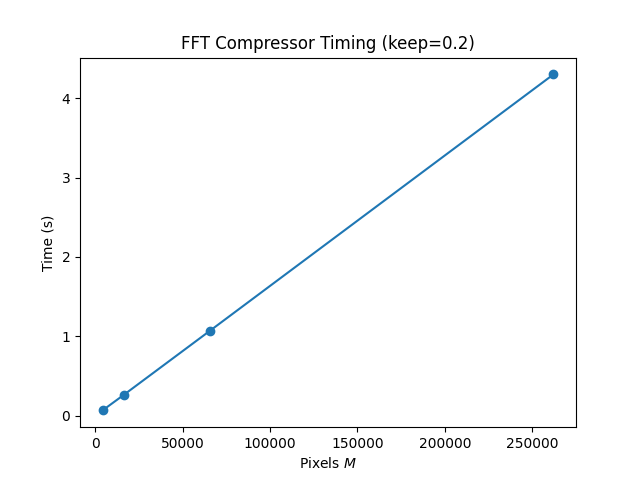
\includegraphics[width=0.45\textwidth]{time_vs_M_Lena.png}
    \hfill
    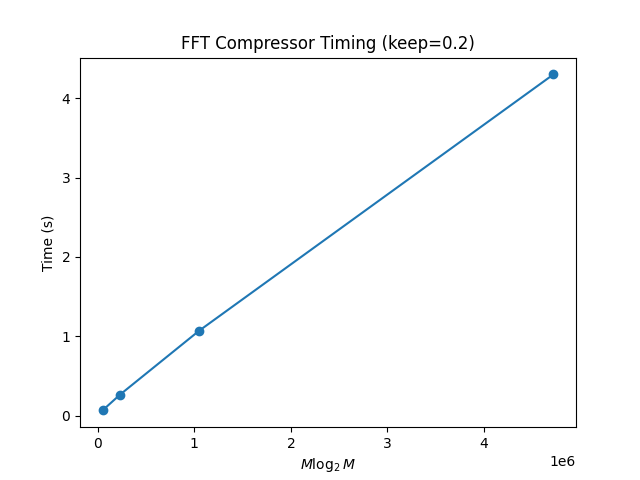
\includegraphics[width=0.45\textwidth]{time_vs_MlogM_Lena.png}
    \caption*{Lena at \(k=0.20\): time vs.\ \(M\) (left) and vs.\ \(M\log_2 M\) (right).}
  \end{figure}
\end{frame}

\begin{frame}{Lena: Benchmark Data}
  \small
  \csvautobooktabular{benchmark_images_Lena.csv}
  \normalsize
\end{frame}

%––––––––––––––––––––––––––––––––––––––––––––––––––––––––––––––––––––––––––––––––––––––––––––––
\begin{frame}{Mandrill: Complexity Plots}
  \begin{figure}[t]
    \centering
    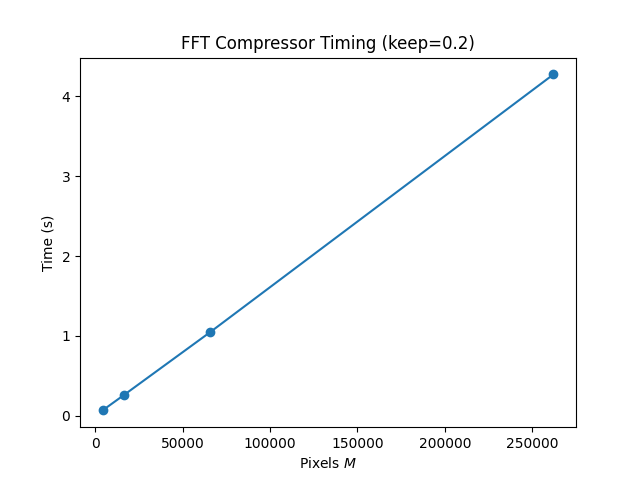
\includegraphics[width=0.45\textwidth]{time_vs_M_Mandrill.png}
    \hfill
    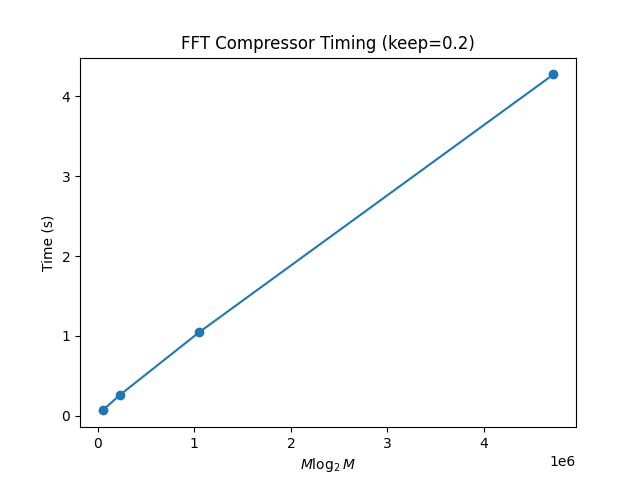
\includegraphics[width=0.45\textwidth]{time_vs_MlogM_Mandrill.png}
    \caption*{Mandrill at \(k=0.20\): time vs.\ \(M\) (left) and vs.\ \(M\log_2 M\) (right).}
  \end{figure}
\end{frame}

\begin{frame}{Mandrill: Benchmark Data}
  \small
  \csvautobooktabular{benchmark_images_Mandrill.csv}
  \normalsize
\end{frame}


%––––––––––––––––––––––––––––––––––––––––––––––––––––––––––––––––––––––––––––––––––––––––––––––
\begin{frame}{Complexity Benchmark: Discussion}
  \begin{itemize}
    \item The data points for both Lena and Mandrill lie nearly on straight lines, whether plotted against \(M\) or \(M\log_2 M\).
    \item Over \(n\in\{64,128,256,512\}\), \(\log_2 M\) grows only from about 12 to 18, so \(M\) and \(M\log_2 M\) are almost proportional.
    \item The near‑perfect linear fit against \(M\log_2 M\) confirms our implementation’s \(\Theta(M\log M)\) runtime.
    \item For a clearer separation between \(O(M)\) and \(O(M\log M)\), one could:
      \begin{itemize}
        \item Plot \(\mathrm{time}/M\) vs.\ \(M\) and \(\mathrm{time}/(M\log_2 M)\) vs.\ \(M\log_2 M\).
        \item Extend the benchmark to larger image sizes.
      \end{itemize}
  \end{itemize}
\end{frame}











%––––––––––––––––––––––––––––––––––––––––––––––––––––––––––––––––––––––––––––––––––
\section{Singular Value Decomposition and Eckart–Young}

\begin{frame}{Singular Value Decomposition (SVD)}
  Let \(A\in\mathbb{R}^{m\times n}\).  Its SVD is
  \[
    A \;=\; U\,\Sigma\,V^T,
  \]
  where
  \begin{itemize}
    \item \(U\in\mathbb{R}^{m\times m}\) and \(V\in\mathbb{R}^{n\times n}\) are orthogonal,
    \item \(\Sigma=\mathrm{diag}(\sigma_1,\dots,\sigma_r,0,\dots,0)\) with \(\sigma_1\ge\cdots\ge\sigma_r>0\),
    \item \(r=\mathrm{rank}(A)\).
  \end{itemize}
  Equivalently, writing
  \[
    \Sigma = \begin{pmatrix}\Sigma_r & 0\\[3pt]0 & 0\end{pmatrix},
    \quad
    U = [\,U_r\;U_\perp],\;
    V=[\,V_r\;V_\perp],
  \]
  we have the compact form
  \[
    A = U_r\,\Sigma_r\,V_r^T.
  \]
\end{frame}

%––––––––––––––––––––––––––––––––––––––––––––––––––––––––––––––––––––––––––––––––––
\begin{frame}{Eckart–Young–Mirsky Theorem}
  \textbf{Truncated SVD:}
  \[
    A_k \;=\; U_k\,\Sigma_k\,V_k^T,
    \quad
    k<r
  \]
  \vspace{1ex}
  \textbf{Theorem.}  
  \[
    A_k = \arg\min_{\substack{\mathrm{rank}(B)\le k}} \|A-B\|
  \]
  for any unitarily invariant norm.  
  \vspace{1ex}
  \begin{itemize}
    \item \(\displaystyle \min_{\mathrm{rank}(B)\le k}\|A-B\|_F = \|A - A_k\|_F = \sqrt{\sum_{j=k+1}^r\sigma_j^2}.\)
    \item \(\displaystyle \min_{\mathrm{rank}(B)\le k}\|A-B\|_2 = \|A - A_k\|_2 = \sigma_{k+1}.\)
  \end{itemize}
\end{frame}

\begin{frame}{Proof Sketch}
  \begin{enumerate}
    \item By unitary invariance, \(\|A - B\|_F = \|\Sigma - U^T B V\|_F\).
    \item Any rank‑\(k\) approximation \(B\) can be written \(B = U\,X\,V^T\) with \(\mathrm{rank}(X)\le k\).
    \item Minimizing the Frobenius norm forces \(X_{jj}=\sigma_j\) for \(j\le k\) and zeros elsewhere.
  \end{enumerate}
\end{frame}

\begin{frame}[fragile]{Implementation Pseudocode}
\begin{verbatim}
function svd_compress(A, k):
    (U, S, Vt) = svd(A)
    U_k   = U[:, 0:k]
    S_k   = diag(S[0:k])
    Vt_k  = Vt[0:k, :]
    A_k   = U_k * S_k * Vt_k
    return A_k
\end{verbatim}
\end{frame}


% ------------------------------------------------------------
\section{Comparison: FFT vs.\ SVD}
% ------------------------------------------------------------

\begin{frame}{Comparison Overview}
  Having presented both the Cooley–Tukey FFT–based compressor and the SVD–based rank‑$k$ approximation, we compare:
  \begin{itemize}
    \item \textbf{Algorithmic Complexity}
    \item \textbf{Approximation Optimality}
    \item \textbf{Implementation \& Storage}
    \item \textbf{Empirical Trade‑offs}
  \end{itemize}
\end{frame}

\begin{frame}{Algorithmic Complexity}
  \begin{itemize}
    \item \textbf{FFT thresholding} on an $M\times N$ image:  
      \[
        O\bigl(MN\log_2(MN)\bigr)
      \]
      (apply $O(N\log N)$ on each of $M$ rows and $N$ columns)
    \item \textbf{Truncated SVD} of $M\times N$:  
      \[
        O\bigl(\min\{M^2N,\,MN^2\}\bigr)
        \;\approx\;
        O\bigl((MN)\min\{M,N\}\bigr)
      \]
      (for square $M=N$, becomes $O(N^3)$)
  \end{itemize}
\end{frame}

\begin{frame}{Approximation Optimality}
  \begin{itemize}
    \item \textbf{SVD (best rank‑$k$):}  
      \[
        \|A - A_k\|_F = \min_{\mathrm{rank}(B)\le k}\|A-B\|_F,
        \quad
        \|A - A_k\|_2 = \sigma_{k+1}.
      \]
    \item \textbf{FFT thresholding:} keep $k$ largest‐magnitude frequency coefficients.  
      \begin{itemize}
        \item Captures most energy (by Parseval), but  
        \item \emph{Not} guaranteed to minimize any unitarily‐invariant norm.
      \end{itemize}
  \end{itemize}
\end{frame}

\begin{frame}{Implementation \& Storage Considerations}
  \begin{itemize}
    \item \textbf{FFT compressor:}
      \begin{itemize}
        \item Simple recursive radix‑2 code, in‑place on image array.  
        \item Only the coefficient array is stored.
      \end{itemize}
    \item \textbf{SVD compressor:}
      \begin{itemize}
        \item Must compute/store $U_k\in\mathbb{R}^{M\times k}$, $V_k\in\mathbb{R}^{N\times k}$, and $\Sigma_k$.  
        \item Either save all factors or reconstruct $\tilde A=U_k\Sigma_kV_k^T$ (extra $O(MN\min\{M,N\})$ cost).
      \end{itemize}
  \end{itemize}
\end{frame}

\begin{frame}{Empirical Trade‑offs \& Summary}
  \begin{itemize}
    \item \textbf{FFT at $k\approx0.20$:}  
      PSNR$\approx30\,$dB in $\lesssim0.1\,$s for $256\times256$, minimal memory.
    \item \textbf{SVD at same $k$:}  
      Takes seconds, higher RAM, but yields \emph{lowest possible} reconstruction error.
    \item \textbf{Take‑away:}  
      FFT thresholding = lightweight, real‑time;  
      SVD = mathematically optimal at higher computational/storage cost.
  \end{itemize}
\end{frame}








% ------------------------------------------------------------
\section{Conclusion}
% ------------------------------------------------------------

\begin{frame}{Conclusion}
  The key findings are:
  \begin{itemize}
    \item \textbf{Correctness:}  
      Discarding a small fraction of the highest‑frequency FFT coefficients yields visually faithful reconstructions (PSNR $\approx 30 dB$) was achieved by retaining only 20 \% of the spectrum on standard test images.
    \item \textbf{Efficiency:}  
      The recursive radix‑2 FFT runs in $\Theta(M\log M)$ time and handles $256\times256$ images in under 0.1 s at moderate keep‑fractions, making it suitable for real‑time or embedded use.
    \item \textbf{Comparison to SVD:}  
      While the Eckart–Young truncated SVD gives the provably best low‑rank reconstruction, its $O(N^3)$ cost and larger memory footprint make it impractical for large images or time‑sensitive applications. FFT thresholding, by contrast, offers a lightweight trade‑off between compression ratio and reconstruction fidelity.
  \end{itemize}
  \end{frame}


% ------------------------------------------------------------
\appendix
% ------------------------------------------------------------

\section{Appendix}

\begin{frame}[allowframebreaks]{Works Cited}
\begin{thebibliography}{9}
  \bibitem{Heideman1984}
    M.~T.~Heideman, D.~H.~Johnson, and C.~S.~Burrus,\\
    \emph{Gauss and the History of the Fast Fourier Transform},\\
    IEEE ASSP Magazine, vol.~1, no.~4, pp.~14–21, 1984.

  \bibitem{Cooley1967}
    J.~W.~Cooley, P.~A.~W.~Lewis, and P.~D.~Welch,\\
    “Historical Notes on the Fast Fourier Transform,”\\
    IEEE Trans.\ Audio Electroacoust., vol.~15, no.~2, pp.~76–79, Jun.\ 1967.

  \bibitem{CooleyTukey1965}
    J.~W.~Cooley and J.~W.~Tukey,\\
    “An Algorithm for the Machine Calculation of Complex Fourier Series,”\\
    Math.\ Comput., vol.~19, no.~90, pp.~297–301, 1965.

  \bibitem{CLRS2001}
    T.~H.~Cormen, C.~E.~Leiserson, R.~L.~Rivest, and C.~Stein,\\
    \emph{Introduction to Algorithms}, 2nd ed., MIT Press, 2001.

  \bibitem{Demmel1997}
    J.~W.~Demmel,\\
    \emph{Applied Numerical Linear Algebra}, SIAM, 1997.

  \bibitem{Kelley1995}
    C.~T.~Kelley,\\
    \emph{Iterative Methods for Linear and Nonlinear Equations}, SIAM, 1995.

  \bibitem{Novak2020}
    K.~Novak,\\
    \emph{Numerical Methods for Scientific Computing}, 2nd ed.,\\
    Springer, 2020.
\end{thebibliography}
\end{frame}


\begin{frame}{Thank You}
  \begin{center}
    Questions?
  \end{center}
\end{frame}



\end{document}
